%!TEX root = ../dissertation.tex
% this file is called up by thesis.tex
% content in this file will be fed into the main document

\graphicspath{{8-conclusions/figures/}}

\chapter{Conclusions and Final Remarks}
\label{ch:conclusions}

\section{Summary and Takeaways}

\begin{itemize}
	\item Dataset matters (highly correlated than images ~\cite{thickstun2018invariances})
	\item Prior knowledge matters in all domains
\end{itemize}


\section{Future Research Directions}

\begin{itemize}
	\item fully-fledged synthesis model
	\item sound as discrete events / sound atoms~\cite{leveau2008atoms}
	\item language model, unsupervised training \cite{huang2018transformer}
	\item Unlimited source of generated model
\end{itemize}


\subsection{A Turing Test for Automatic Music Transcription}

Finally, a consideration is needed for the fundamental limitation on any music transcription task, either automatic or manual, and when it can be said that AMT is solved.
Polyphonic music contains a mixture of sounds with an indefinite number of notes being played simultaneously; even the most experienced musicians may not be able to identify every note, and the audio mixture may not contain the sufficient information to convey all notes in the first place.
It would be unreasonable to expect anyone to perfectly transcribe all notes in the score of an orchestral music from an audio file, but it would be sensible for a trained musician to produce a version of score that, when played by the same orchestra, sounds indistinguishable to the original recording.
Considering these limitations, passing this ``transcriptional Turing test'' as shown in Figure \ref{fig:turing}, rather than achieving the 100\% accuracy on a certain dataset, should be the ultimate goal of automatic music transcription, at which point it can be said to have a human-level intelligence on this task.

\begin{figure}
	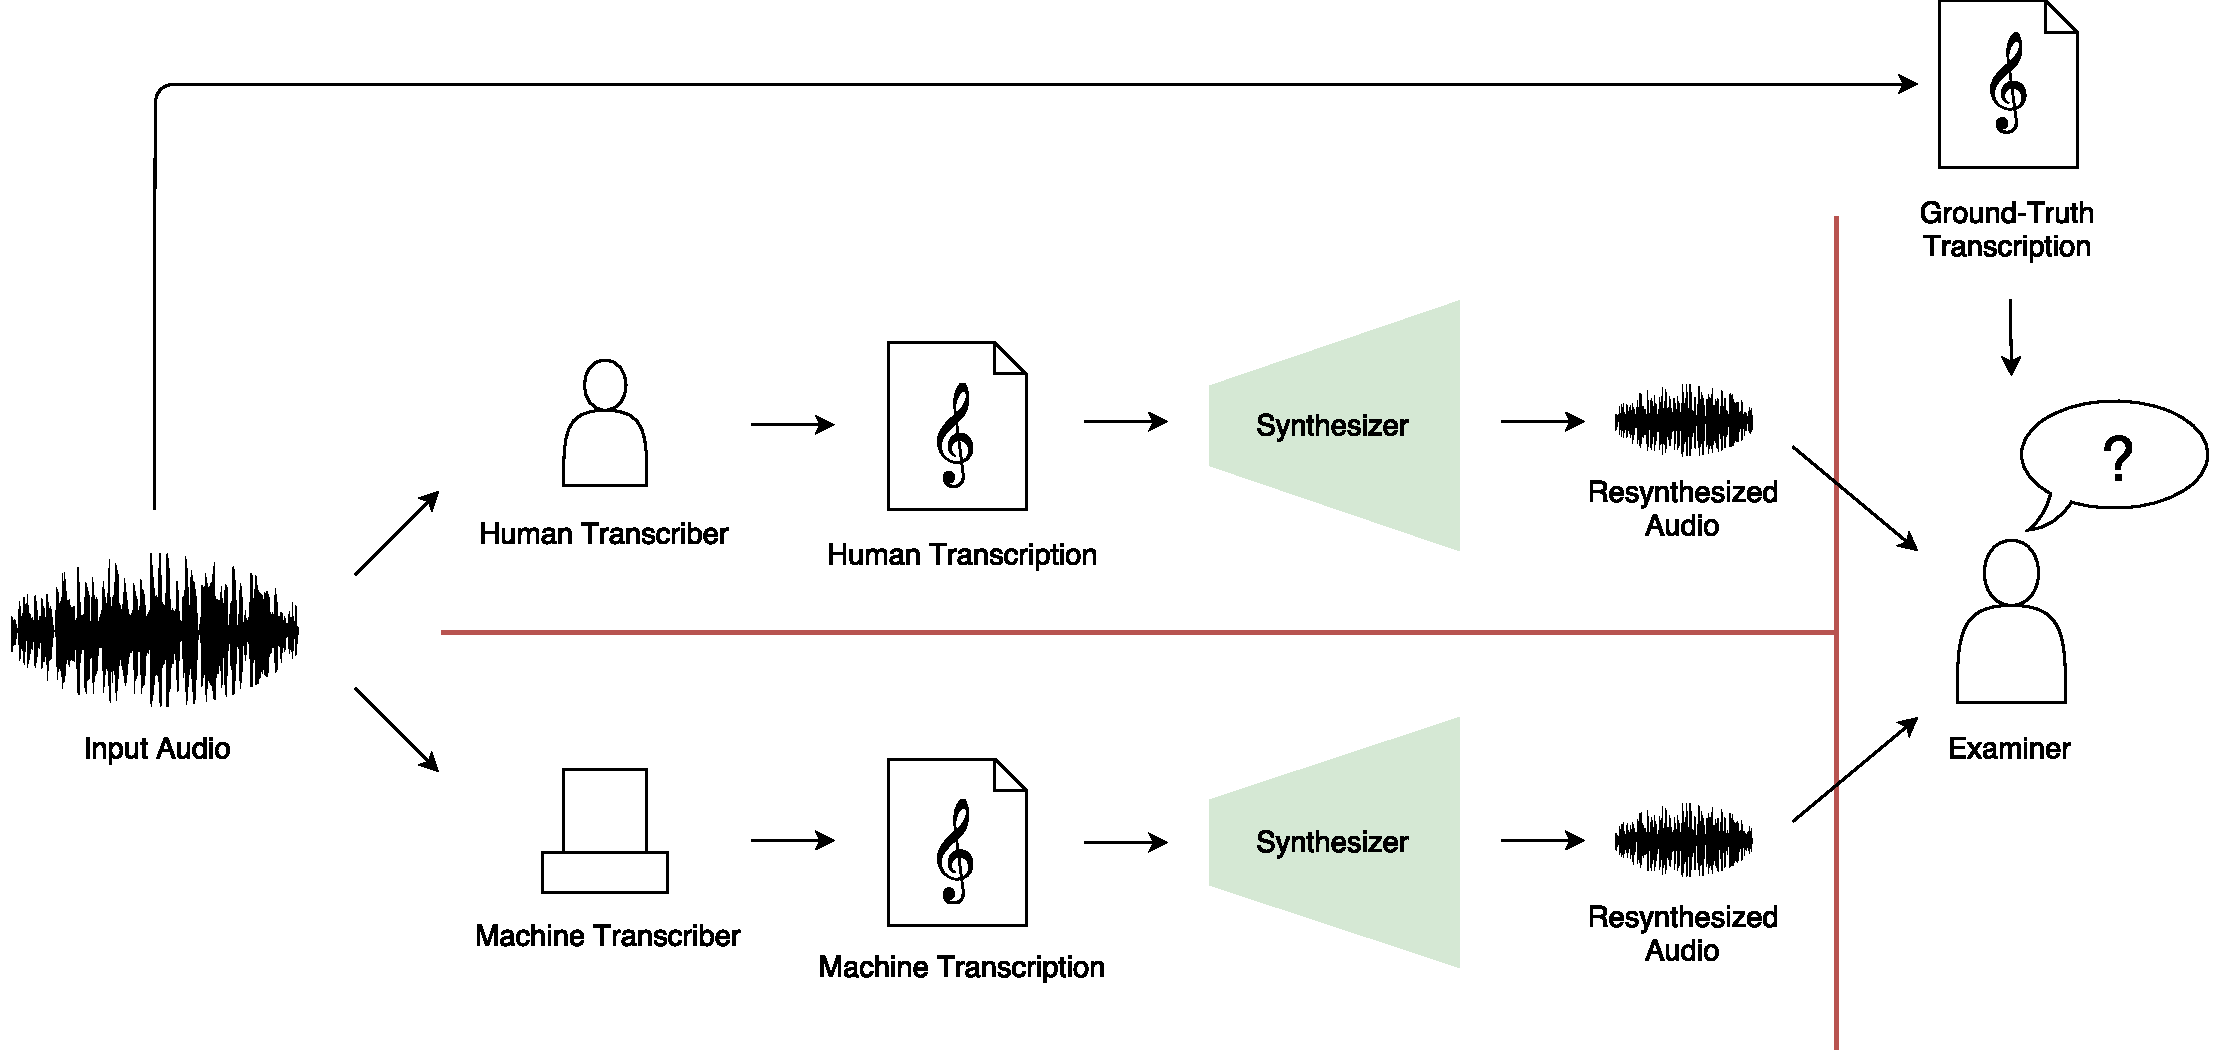
\includegraphics[width=\textwidth]{turing.pdf}
	\caption{The \emph{transcriptional Turing test}, to test whether an automatic music transcription algorithm has reached human-level. While this provides some conceptual insights to the adversarial training setup, to be covered in the later chapters, fully achieving the human-level performance is out of scope of this thesis.}
	\label{fig:turing}
\end{figure}

\section{Conclusions}

\pagebreak